\documentclass[11pt]{report}
\usepackage[utf8]{inputenc} % set input encoding (not needed with XeLaTeX) 
%%% PAGE DIMENSIONS                                                        
\usepackage{geometry} % to change the page dimensions                     
\geometry{a4paper} % or letterpaper (US) or a5paper or....                 
\usepackage{graphicx} % support the \includegraphics command and options   
% \usepackage[parfill]{parskip} % Activate to begin paragraphs with an empty line rather than an indent  
%%% PACKAGES
\usepackage{booktabs} % for much better looking tables
\usepackage{array} % for better arrays (eg matrices) in maths
\usepackage{paralist} % very flexible & customisable lists (eg. enumerate/itemize, etc.)
\usepackage{verbatim} % adds environment for commenting out blocks of text & for better verbatim
\usepackage{subfig} % make it possible to include more than one captioned figure/table in a single float
\usepackage[francais]{babel}
\usepackage{textcomp}
\usepackage{hyperref}
\usepackage{lscape}
\usepackage{calc}
\usepackage{xcolor}
\usepackage{pdflscape}
% These packages are all incorporated in the memoir class to one degree or another...

%%% HEADERS & FOOTERS                                                         
\usepackage{fancyhdr} % This should be set AFTER setting up the page geometry 
\pagestyle{fancy} % options: empty , plain , fancy           
\renewcommand{\headrulewidth}{1pt} % customise the layout... 
\fancyhead[L]{\leftmark}
\fancyhead[R]{Manuel Cultibox}
\renewcommand{\footrulewidth}{1pt}
\fancyfoot[L]{
\includegraphics[scale=0.3]{./wiki/img/logo_seul.png}}
\fancyfoot[C]{Green Box SAS}
\fancyfoot[R]{\textbf{page \thepage}}
\setlength{\headheight}{15pt}
%%% Definition de la profondeur de la numerotation
\setcounter{secnumdepth}{7}
\setcounter{tocdepth}{7}

%%% Command
\newlength{\imgwidth}
\newcommand\scalegraphics[1]{%
    \settowidth{\imgwidth}{\includegraphics{#1}}%
    \setlength{\imgwidth}{\minof{\imgwidth}{0.9\textwidth}}%
    \includegraphics[width=\imgwidth]{#1}%
}
%%% SECTION TITLE APPEARANCE    
\usepackage{sectsty}            
\allsectionsfont{\sffamily\mdseries\upshape} % (See the fntguide.pdf for font help)  
% (This matches ConTeXt defaults)   

%%% ToC (table of contents) APPEARANCE 
\usepackage[nottoc,notlof,notlot]{tocbibind} % Put the bibliography in the ToC 
\usepackage[titles,subfigure]{tocloft} % Alter the style of the Table of Contents
\renewcommand{\cftsecfont}{\rmfamily\mdseries\upshape}
\renewcommand{\cftsecpagefont}{\rmfamily\mdseries\upshape} % No bold!

%%% END Article customizations
%%% The "real" document content comes below...
\title{Manuel d'utilisation de la Cultibox}
\author{Cultibox}
\begin{document}
\makeatletter
  \begin{titlepage}             
    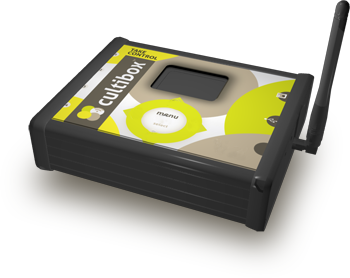
\includegraphics{./wiki/img/box_3d_1.png}      
    \vskip 1pt
    \Huge                               
    Manuel d'utilisation de la Cultibox
    \vskip 5pt

    \hrule{}\hrule{}\hrule{}\hrule{}
    \hrule{}\hrule{}\hrule{}\hrule{}
    \begin{flushright}
    {\large\textbf{\@date}}
    \vskip 1pt
    {\large\textbf{Green Box SAS}}
    \vskip 1pt
    {\large\textbf{8 Rue Marceau}}
    \vskip 1pt
    {\large\textbf{38000 Grenoble}}
    \end{flushright}
    \vfill
    \begin{center}
    
\includegraphics[scale=1.5]{./wiki/img/logo_seul.png}
    \end{center}
    \date\today
  \end{titlepage}
\makeatother

\newpage
\tableofcontents 
\input{./wiki_tex/quick_guide}
\input{./wiki_tex/Introduction}
\input{./wiki_tex/general_caution}
\input{./wiki_tex/contents}
\input{./wiki_tex/sav}
\input{./wiki_tex/recyclage}
\input{./wiki_tex/fabrication}
\input{./wiki_tex/install}
\input{./wiki_tex/install_windows}
\input{./wiki_tex/install_mac}
\input{./wiki_tex/install_linux}
\input{./wiki_tex/install_Plug}
\input{./wiki_tex/install_sensor}
\input{./wiki_tex/interface_logiciel}
\input{./wiki_tex/gui_soft_welcome}
\input{./wiki_tex/gui_soft_conf}
\input{./wiki_tex/gui_soft_logs}
\input{./wiki_tex/gui_soft_prog}
\input{./wiki_tex/gui_soft_prog_regul}
\input{./wiki_tex/gui_soft_second_regul}
\input{./wiki_tex/gui_soft_plugs}
\input{./wiki_tex/gui_soft_cost}
\input{./wiki_tex/gui_soft_cal}
\input{./wiki_tex/gui_soft_cal_lunar}
\input{./wiki_tex/gui_soft_cal_engrais}
\input{./wiki_tex/gui_soft_wizard}
\input{./wiki_tex/gui_soft_historic}
\input{./wiki_tex/gui_box}
\input{./wiki_tex/gui_box_start}
\input{./wiki_tex/gui_box_main}
\input{./wiki_tex/gui_box_menu}
\input{./wiki_tex/gui_box_menu_logs}
\input{./wiki_tex/gui_box_menu_programme}
\input{./wiki_tex/gui_box_menu_calendar}
\input{./wiki_tex/gui_box_menu_param}
\input{./wiki_tex/gui_box_menu_param_culti}
\input{./wiki_tex/gui_box_menu_param_emettor}
\input{./wiki_tex/gui_box_menu_param_sensor}
\input{./wiki_tex/other}
\input{./wiki_tex/faq}
\input{./wiki_tex/pts}
\input{./wiki_tex/advance}
\input{./wiki_tex/declaration_ce}
\end{document}

